\documentclass[9pt, aspectratio=169]{beamer}
\usepackage{FiraSans}
\usetheme{metropolis}
\usepackage[utf8]{inputenc}
\usepackage{amsmath}
\usepackage{amsfonts}
\usepackage{amssymb}
\usepackage{multicol}
\usepackage{tikz}
\usetikzlibrary{matrix}
\usepackage{xcolor}
\usepackage[T1]{fontenc} 
\usepackage[skins]{tcolorbox}
\author{Nicola Roman\`o - nicola.romano@ed.ac.uk}
\title{Lecture 4 - Filters}
\setlength{\fboxsep}{0pt}
\setbeamertemplate{caption}{\raggedright\insertcaption\par}
\setbeamertemplate {footline}{\begin{scriptsize}\hfill\insertframenumber ~of \inserttotalframenumber\kern1em\vskip5pt\end{scriptsize}}

%\setbeamercovered{transparent} 
%\setbeamertemplate{navigation symbols}{} 

\titlegraphic{\centering 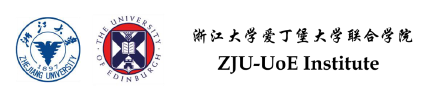
\includegraphics[scale=.5]{instituteLogo.png}}
\date{}

\AtBeginSection[]
{
  \begin{frame}<beamer>
    {Outline}
    \huge{\tableofcontents[currentsection]}
  \end{frame}
}

\begin{document}

\newtcolorbox{codebox}{enhanced,
    top=2pt,
    left=2pt,
    right=2pt,
    bottom=2pt,
    boxrule=0pt,
    leftrule=5pt,
    sharp corners,
    colback=gray!20,
    colframe=blue!60!black}

\begin{frame}
    \titlepage
\end{frame}

\begin{frame}
    {Learning objectives}
    \begin{columns}
        \begin{column}{0.8\textwidth}
            \begin{itemize}
                \item Define rank and convolutional filters
                \item Explain their use in image analysis
                \item Implement basic filters in Python
            \end{itemize}
        \end{column}
        \begin{column}{0.2\textwidth}
            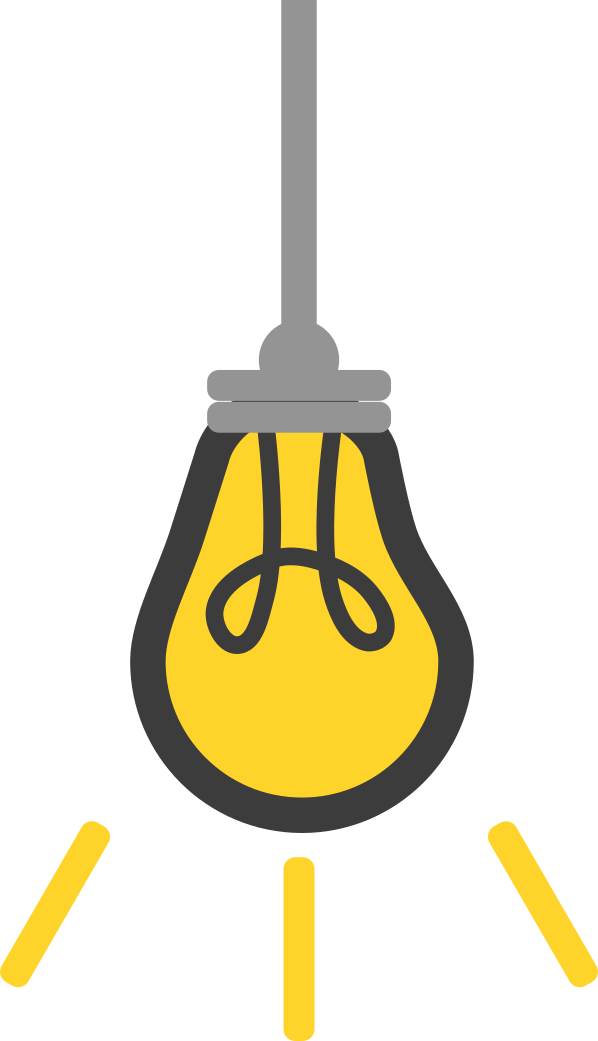
\includegraphics[angle=-30, origin=tr, width=1.5\textwidth]{lightbulb.png}
        \end{column}
    \end{columns}
\end{frame}

\begin{frame}
    {Types of pixel operations}
    Operations for manipulating pixel intensities

    Two types of operations:
    \begin{itemize}
        \item Point operations - Change pixel intensity based only on its value - $I'_{(x, y)} = f(I_{x, y})$ (see Lecture 3)
        \item \textbf{Neighbourhood operations} - Change pixel intensity based on the intensity of the pixel and its neighbours.
    \end{itemize}
\end{frame}

\begin{frame}
    {Filters}
    Neighbourhood operations, often called \textbf{filters} allow to modify an image in a way that is not possible with point operations.

    \begin{itemize}
        \item Detect simple structures such as edges, corners, lines, etc.
        \item Perform operations such as smoothing, sharpening, etc.
        \item Noise reduction
    \end{itemize}
    \pause
    Today we will look at:
    \begin{itemize}
        \item \textbf{Rank filters} - the new pixel value is a function of the rank of the pixel values of the neighbourhood
        \item \textbf{Convolutional filters} - the new pixel value is a weighted sum of the pixel values of the neighbourhood
    \end{itemize}

\end{frame}

\section{Rank filters}

\begin{frame}
    {Rank filters}
    \begin{columns}
        \begin{column}{.5\textwidth}
            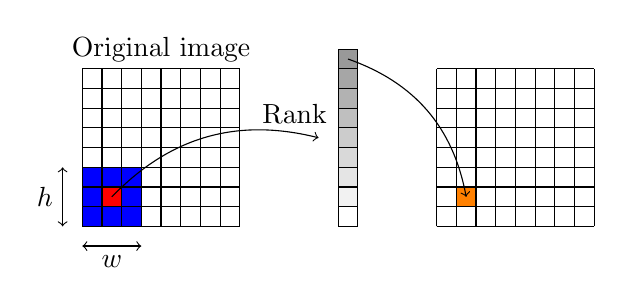
\begin{tikzpicture}[scale=0.25]
                \draw [fill=blue] (0, 0) rectangle (3, 3);
                \draw (0, 0) grid (8, 8);
                \draw (4, 9) node {Original image};
                \draw [fill=red] (1, 1) rectangle (2, 2);
                \draw [<->] (0, -1) -- (3, -1) node[below, pos=0.5] {$w$};
                \draw [<->] (-1, 0) -- (-1, 3) node[left, pos=0.5] {$h$};

                \foreach \i in {0,10,...,80}                    \draw [fill=gray!\i] (13, \i/10) rectangle (14, \i/10 + 1);

                \path[->] (1.5, 1.5) edge[bend left=30] node[above, pos=0.9] {Rank} (12, 4.5);

                \draw (18, 0) grid (26, 8);
                \draw [fill=orange] (19, 1) rectangle (20, 2);
                \path[->] (13.5, 8.5) edge[bend left=30] (19.5, 1.5);
            \end{tikzpicture}
        \end{column}
        \begin{column}{.5\textwidth}
            \begin{itemize}
                \item We decide on a window size $w \times h$ (other non-rectangular shapes are possible)
                \item We traverse each pixel in the image and take its $w \times h$ neighbourhood
                \item We rank the intensity of each pixel in the neighbourhood
                \item We take a specific value (e.g. minimum, maximum, median) and set the output value to this value
            \end{itemize}
        \end{column}
    \end{columns}
\end{frame}

\begin{frame}
    {Example - median filter}
    \centering
    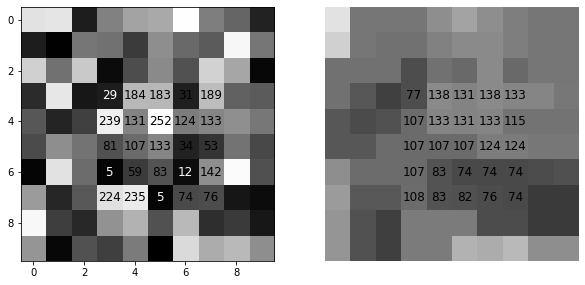
\includegraphics[width=.8\textwidth]{median_filter_example.png}
\end{frame}

\begin{frame}
    {Rank filters in Scikit Image}
    Rank filters are implemented in Scikit Image in the `skimage.rank` module.\\
    These filters require a \textit{footprint} of the pixel neighbourhood, as a matrix of 0 and 1.

    For example

    \begin{codebox}
        \texttt{from skimage.rank import median\\
            \\
            \# 3x3 neighbourhood\\
            footprint = np.ones(3, 3)\\
            img\_median = median(img, selem=footprint)
        }
    \end{codebox}
    \centering
    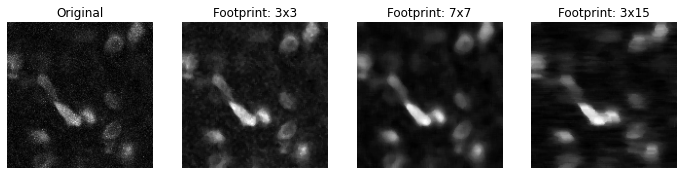
\includegraphics[width=.85\textwidth]{median_filter_different_footprints.png}
\end{frame}

\begin{frame}
    {Non-rectangular footprints}
    The footprint can be a \textit{non-rectangular} matrix. For example, you can generate a \textbf{circular} shape using the \texttt{skimage.morphology.disk} function or a \textbf{diamond} shape using the \texttt{skimage.morphology.diamond} function.\\

    \vspace{2em}

    \begin{columns}
        \begin{column}{.5\textwidth}
            \begin{codebox}
                \texttt{from skimage.morphology import disk, diamond\\
                    \\
                    dsk = disk(7) \# A disk, radius 7\\
                    dia = diamond(7) \# A diamond, radius 7\\
                    \\
                    fig, ax = plt.subplots(1, 2)\\
                    ax[0].imshow(dsk, cmap="gray")\\
                    ax[1].imshow(dia, cmap="gray")
                }
            \end{codebox}
        \end{column}
        \begin{column}{.5\textwidth}
            \centering
            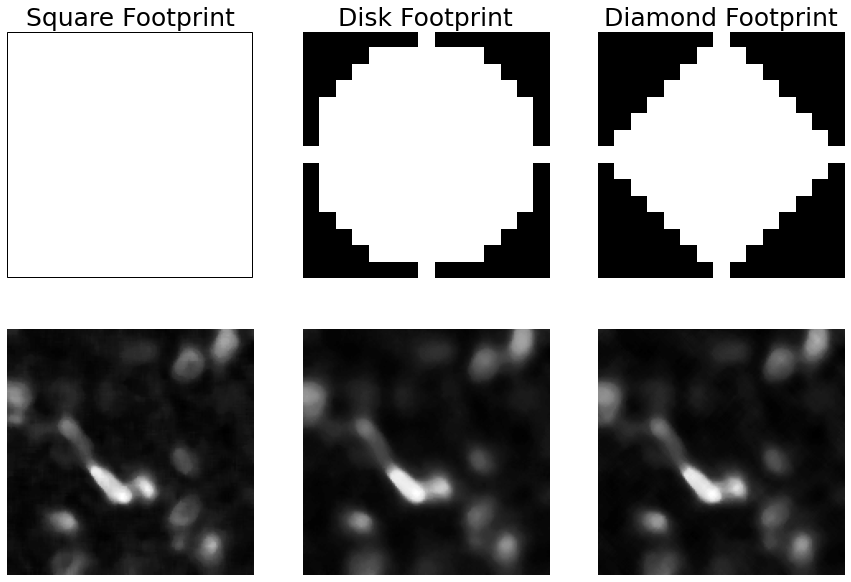
\includegraphics[width=\textwidth]{different_shaped_footprints.png}
        \end{column}
    \end{columns}
\end{frame}

\begin{frame}
    {Rank filters - use cases}
    Rank filters are very simple, but have useful applications.\\

    The \textbf{median filter} is used to remove noise and to smooth images.\\
    \pause
    \vspace{1em}
    The \textbf{maximum filter} can be used in binary images to remove  small "holes". It is also a very common filter used in modern neural networks for image analysis.\\
    \only<2>{
        \centering
        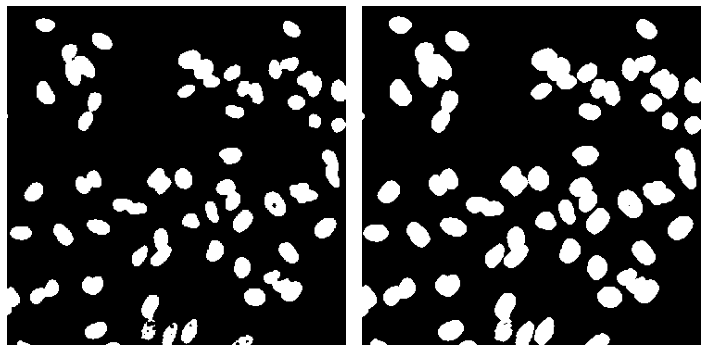
\includegraphics[width=.55\textwidth]{maximum_filter.png}
    }
    \only<3>{
        \begin{flushleft}
            The \textbf{minimum filter} can be used to remove small bright spots.
        \end{flushleft}
        \centering
        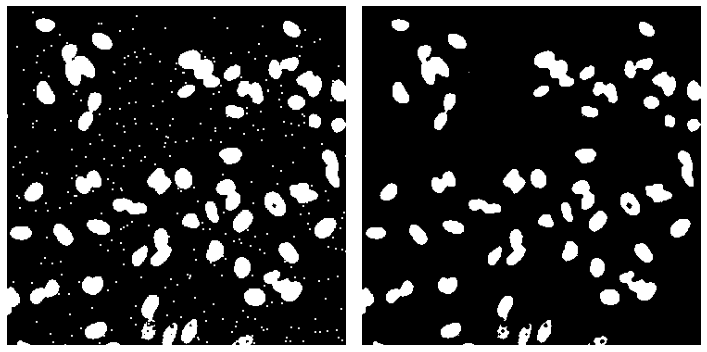
\includegraphics[width=.55\textwidth]{minimum_filter.png}
    }
\end{frame}

\section{Convolutional filters}

\begin{frame}
    {Convolutional filters}
    A \textbf{convolutional filter} consists of a small matrix, called a \textbf{kernel}, that is used to process an image.\\

    Convolution takes each pixel of the image together with its neighbours and adds them together, weighting each neighbour by the value of a kernel of the same size of the neighbourhood.

\end{frame}

\begin{frame}
    {Example of a convolutional filter}
    \centering
    \only<1>{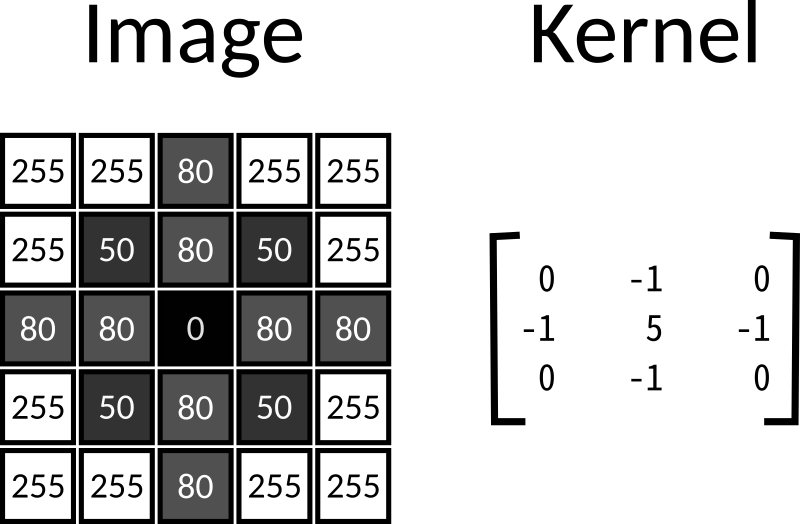
\includegraphics[width=.7\textwidth]{image_kernel.png}}
    \only<2>{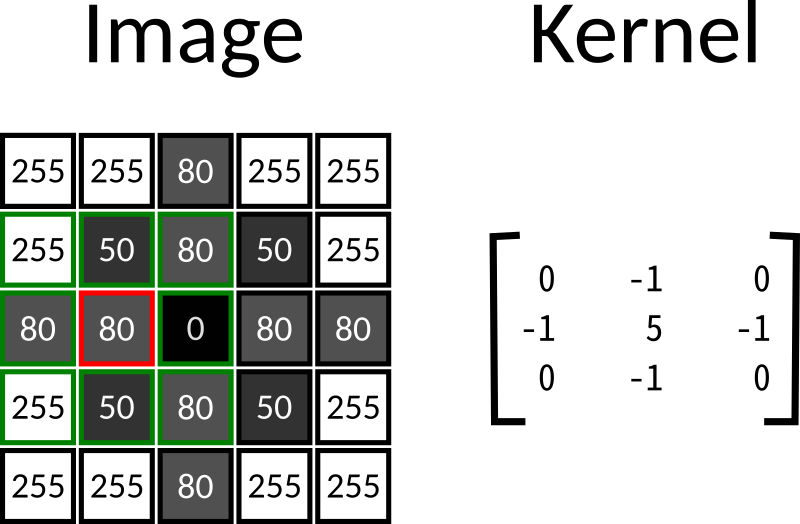
\includegraphics[width=.7\textwidth]{image_kernel_sel.png}\\
        The convolved pixel value will be
        $$255*0+50*(-1)+80*0+80*(-1)+80*5+0*(-1)+255*0+50*(-1)+80*0 = \textbf{220}
        $$
    }
\end{frame}

\begin{frame}
    {Example of a convolutional filter - result}
    \centering
    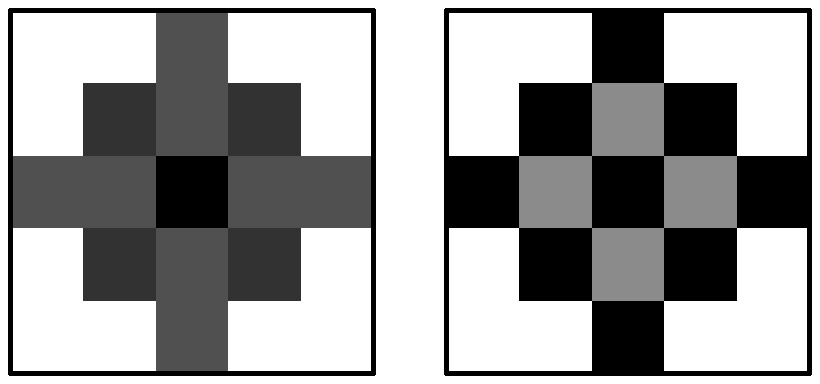
\includegraphics[width=.6\textwidth]{example_filter_before_after.png}\\

    Our image, after applying the convolutional filter.

    \pause
    \vspace{1em}
    Convolutional filters are \textbf{shift invariant}, meaning the result of the convolution is the same regardless of the position of the pixel in the original image (as long as it has the same neighbourhood).

\end{frame}

\begin{frame}
    {Common convolutional filters - averaginig filter}
    The \textbf{averaging filter} or \textbf{box blur} is a simple filter that is used to reduce noise in an image.\\

    It simply takes the average of the pixel values in the neighbourhood.

    \begin{columns}
        \begin{column}{.25\textwidth}
            \centering
            Example 3x3 kernel:\\
            $$\begin{bmatrix}1/9&1/9&1/9\\1/9&1/9&1/9\\1/9&1/9&1/9\end{bmatrix}$$
        \end{column}
        \begin{column}{.75\textwidth}
            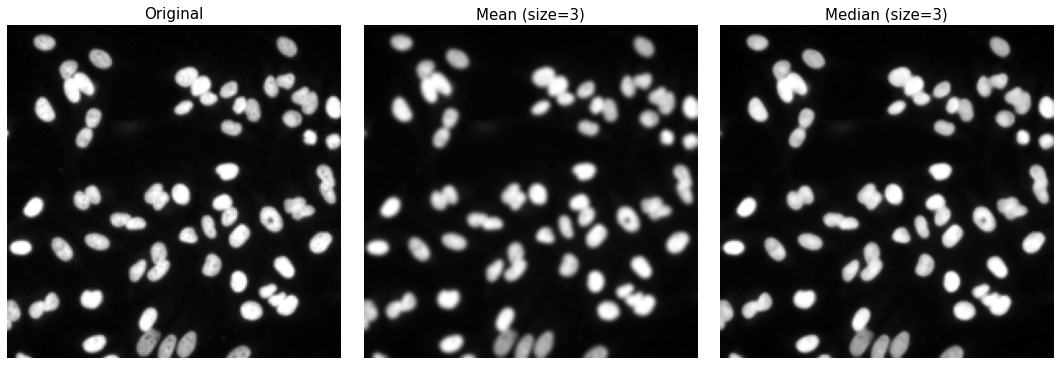
\includegraphics[width=\textwidth]{mean_vs_median.png}
        \end{column}
    \end{columns}

    Not as good as the \textbf{median filter}, as it is sensitive to outliers and does not preserve edges as well (can you get an intuition as to why?).

\end{frame}

\begin{frame}
    {Common convolutional filters - Gaussian filter}
    The \textbf{Gaussian filter} is a filter that is used to smooth images.\\

    It uses a \textbf{Gaussian} function to weight the pixel values in the neighbourhood.\\

    \vspace{2em}

    \begin{columns}
        \begin{column}{.3\textwidth}
            \centering
            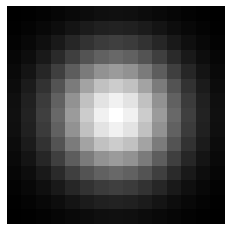
\includegraphics[width=.5\textwidth]{gaussian.png}

            \vspace{2em}

            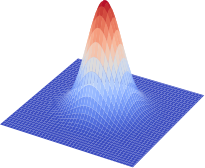
\includegraphics[width=.5\textwidth]{gaussian3D.png}
        \end{column}
        \begin{column}{.7\textwidth}
            \begin{Large}
                $$G_\sigma = \frac{1}{2\pi\sigma^2}e^{-\frac{(x^2+y^2)}{2\sigma^2}}$$
            \end{Large}

            \centering
            Example of gaussian kernels 3x3 and 5x5 (approx.):

            $$\frac{1}{16}\begin{bmatrix}1&2&1\\2&4&2\\1&2&1\end{bmatrix} \qquad
                \frac{1}{256}\begin{bmatrix}1&4&6&4&1\\4&16&24&16&4\\6&24&36&24&6&\\4&16&24&16&4&\\1&4&6&4&1\end{bmatrix}$$
        \end{column}
    \end{columns}
\end{frame}

\begin{frame}
    {Common convolutional filters - Gaussian filter - result}
    Example of gaussian filters with increasing sigma values:

    \centering
    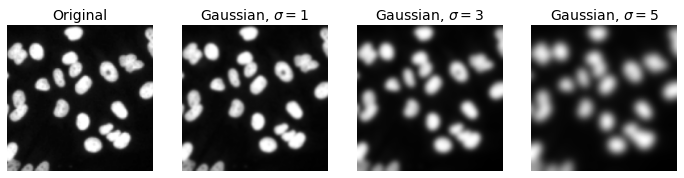
\includegraphics[width=\textwidth]{gaussian_filter_example.png}

    Gaussian filters result in a blurring effect, which can be useful for removing noise, or in general removing the finer detail of the image (low-pass filtering).

    \begin{codebox}
        \texttt{from skimage.filters import gaussian\\
            img\_blurred = gaussian(image, sigma=1)
        }
    \end{codebox}
\end{frame}

\begin{frame}
    {Sharpening filters}
    Sharpening filters are used to increase the detail of an image.\\

    \only<1>{
        \centering
        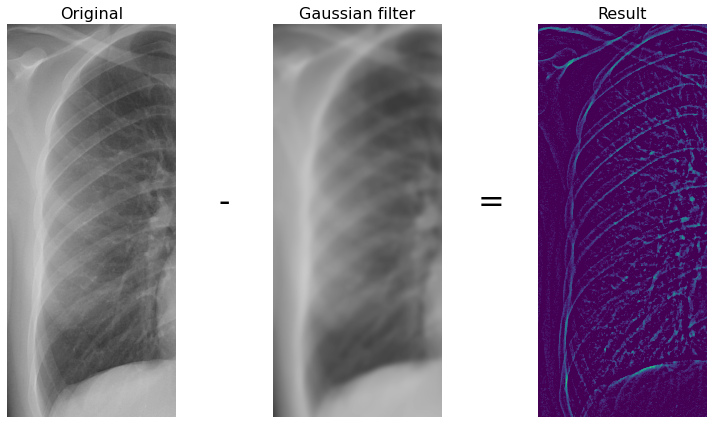
\includegraphics[width=.7\textwidth]{sharpening_get_details.png}

        If we apply a Gaussian filter to the image we will remove detail, so if we subtract the result from the original image we will get the "details" of the image.
    }
    \only<2>{
        \centering
        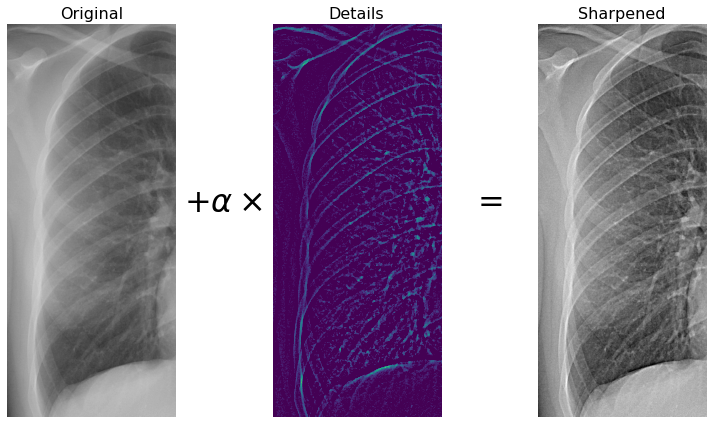
\includegraphics[width=.7\textwidth]{sharpening_add_details.png}

        We can now add the details to the original image, thus sharpening it!

        This process is called \textbf{"unsharp masking"}.
    }
\end{frame}

\begin{frame}
    {Unsharp masking in Scikit Image}
    You can use the \texttt{skimage.filters.unsharp\_mask} function to apply unsharp masking to images.

    \begin{columns}
        \begin{column}{.65\textwidth}
            \begin{codebox}
                \small{
                    \texttt{from skimage.filters import unsharp\_mask\\
                        img\_sharpened = unsharp\_mask(img, radius=15, amount=2)
                    }
                }
            \end{codebox}
            \vspace{2em}
            \onslide<2>{
                \textbf{Exercise:} try writing your own unsharp masking function.\\
                It should accept an image, a radius (the $\sigma$ of the gaussian blur) and an amount for sharpening and return the sharpened image.
            }
        \end{column}
        \begin{column}{.35\textwidth}
            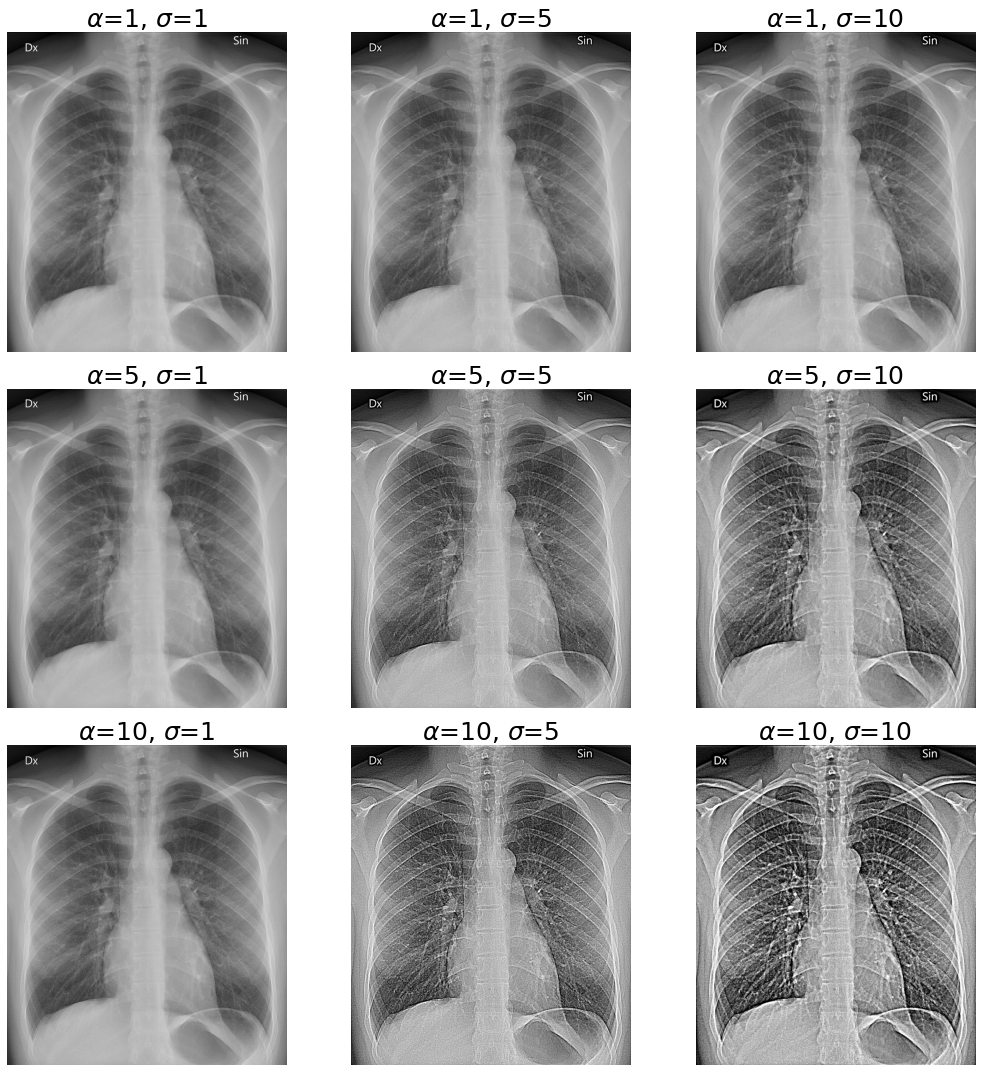
\includegraphics[height=.7\textheight]{unsharp_mask_parameter_space.png}
            \tiny{\color{gray}{Exploring the parameter space of unsharp masking.}\color{black}}
        \end{column}
    \end{columns}
\end{frame}

\begin{frame}
    {What happens at the edges?}
    Convolutional filters traverse the image pixel by pixel and apply a function that takes into account the pixel's neighbourhood.\\

    \textbf{What happens at the edges}, where the neighbourhood is not complete?\\

    There are several ways to deal with this.
    \pause
    \footnotesize{
        \begin{itemize}
            \item<2->\textbf{Zero-pad the image}: we create an extra padding of pixels with a value of zero around the image.
            \item<3-> \textbf{Extend the image}: edge pixels are copied, corner pixels are repeated as \textit{wedges}.
            \item<4-> \textbf{Wrap the image}: extra pixels are taken from the opposite side of the image.
            \item<5-> \textbf{Mirror the image}: extra pixels are created by mirroring the image.
            \item<6-> \textbf{Crop the image}: we ignore the edge pixels. This will result in a smaller output image.
            \item<6-> \textbf{Crop the kernel}: we only use the kernel values corresponding to a pixel in the image. Kernel weights are adjusted to account for this.
        \end{itemize}
    }
    \onslide<2->{
        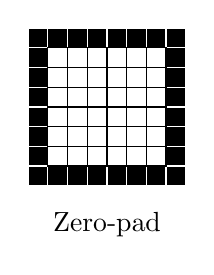
\begin{tikzpicture}[scale=.25]
            \draw [fill=black] (-1, -1) rectangle (7, 7);
            \draw [color=white] (-1, -1) grid (7, 7);
            \draw [fill=white] (0, 0) rectangle (6, 6) grid (0, 0);
            \node at (3, -3) {Zero-pad};
        \end{tikzpicture}
    }
    \onslide<3->{
        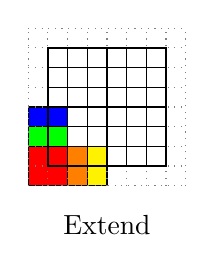
\begin{tikzpicture}[scale=.25]
            \draw [fill=red] (-1, -1) rectangle (1, 1);
            \draw [fill=orange] (1, -1) rectangle (2, 1);
            \draw [fill=yellow] (2, -1) rectangle (3, 1);
            \draw [fill=green] (-1, 1) rectangle (1, 2);
            \draw [fill=blue] (-1, 2) rectangle (1, 3);

            \draw [color=gray, dotted] (-1, -1) grid (7, 7);
            \draw [thick] (0, 0) rectangle (6, 6);
            \draw [thin] (0, 0) grid (6, 6);

            \node at (3, -3) {Extend};
        \end{tikzpicture}
    }
    \onslide<4->{
        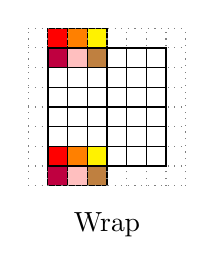
\begin{tikzpicture}[scale=.25]
            \draw [fill=red] (0, 0) rectangle (1, 1);
            \draw [fill=orange] (1, 0) rectangle (2, 1);
            \draw [fill=yellow] (2, 0) rectangle (3, 1);
            \draw [fill=red] (0, 6) rectangle (1, 7);
            \draw [fill=orange] (1, 6) rectangle (2, 7);
            \draw [fill=yellow] (2, 6) rectangle (3, 7);

            \draw [fill=purple] (0, 5) rectangle (1, 6);
            \draw [fill=pink] (1, 5) rectangle (2, 6);
            \draw [fill=brown] (2, 5) rectangle (3, 6);
            \draw [fill=purple] (0, 0) rectangle (1, -1);
            \draw [fill=pink] (1, 0) rectangle (2, -1);
            \draw [fill=brown] (2, 0) rectangle (3, -1);

            \draw [color=gray, dotted] (-1, -1) grid (7, 7);
            \draw [thick] (0, 0) rectangle (6, 6);
            \draw [thin] (0, 0) grid (6, 6);

            \node at (3, -3) {Wrap};
        \end{tikzpicture}
    }
    \onslide<5->{
        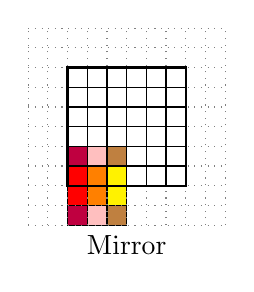
\begin{tikzpicture}[scale=.25]
            \draw [fill=red] (0, -1) rectangle (1, 1);
            \draw [fill=orange] (1, -1) rectangle (2, 1);
            \draw [fill=yellow] (2, -1) rectangle (3, 1);
            \draw [fill=purple] (0, 1) rectangle (1, 2);
            \draw [fill=pink] (1, 1) rectangle (2, 2);
            \draw [fill=brown] (2, 1) rectangle (3, 2);
            \draw [fill=purple] (0, -2) rectangle (1, -1);
            \draw [fill=pink] (1, -2) rectangle (2, -1);
            \draw [fill=brown] (2, -2) rectangle (3, -1);

            \draw [color=gray, dotted] (-2, -2) grid (8, 8);
            \draw [thick] (0, 0) rectangle (6, 6);
            \draw [thin] (0, 0) grid (6, 6);

            \node at (3, -3) {Mirror};
        \end{tikzpicture}
    }
    \onslide<6->{
        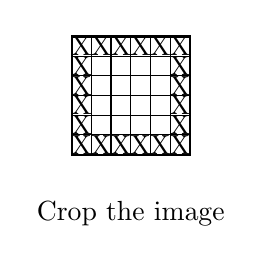
\begin{tikzpicture}[scale=.25]
            \foreach \i in {0.5,1.5,...,5.5}
                {
                    \node at (\i, 0.5) {X};
                    \node at (\i, 5.5) {X};
                }
            \foreach \i in {1.5,2.5,3.5,4.5}
                {
                    \node at (0.5, \i) {X};
                    \node at (5.5, \i) {X};
                }
            \draw [thick] (0, 0) rectangle (6, 6);
            \draw [thin] (0, 0) grid (6, 6);

            \node at (3, -3) {Crop the image};
        \end{tikzpicture}
    }
    \onslide<6->{
        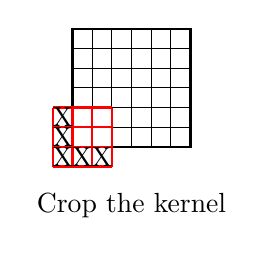
\begin{tikzpicture}[scale=.25]
            \draw [thick] (0, 0) rectangle (6, 6);
            \draw [thin] (0, 0) grid (6, 6);
            \draw [thick, color=red] (-1, -1) grid (2, 2);
            \node at (-0.5, 1.5) {X};
            \node at (-0.5, 0.5) {X};
            \node at (-0.5, -0.5) {X};
            \node at (0.5, -0.5) {X};
            \node at (1.5, -0.5) {X};

            \node at (3, -3) {Crop the kernel};
        \end{tikzpicture}
    }
\end{frame}

\begin{frame}
{Edge behaviour in Scikit Image}
Filters in Scikit Image allow you to choose what to do with the edge pixels using the \texttt{mode} parameter.

For example

\begin{codebox}
\texttt{from skimage.filters import gaussian\\
image\_smoothed = gaussian(image, sigma=1, mode="mirror")}
\end{codebox}

Allowed values for \texttt{mode} are

\begin{itemize}
\item \texttt{constant} - padding with the value specified by \texttt{cval}
\item \texttt{nearest} - extend
\item \texttt{mirror} and \texttt{reflect} - both of these mirror the image, but \texttt{reflect} does not duplicate the edge pixel
\item \texttt{wrap}
\end{itemize}

\end{frame}

\begin{frame}
{Want to try out more?}

You can design your own convolutional filter and apply it to an image using the \texttt{skimage.filters.edges.convolve} function.

What happens using this kernel?

$$\begin{bmatrix}0 & 0 & 0 \\ 0 & 1 & 0 \\ 0 & 0 & 0\end{bmatrix}$$

What about this?

$$\begin{bmatrix}0 & 0 & 0 \\ 0 & 1.5 & 0 \\ 0 & 0 & 0\end{bmatrix}$$

You can see convolutional filters in action at \href{https://setosa.io/ev/image-kernels/}{\underline{this website}}.
\end{frame}

\begin{frame}
{Summary}
\begin{itemize}
\item Image filters are a simple yet powerful way of manipulating images.
\item Filters can be used to remove noise, smooth images, sharpen them, and more.
\item Rank filters such as median, maximum and minimum work by choosing a specific value of the pixels in the neighbourhood, depending on their rank.
\item Convolutional filters use a kernel to apply a linear transformation to the image.
\item In the next lecture we will look at using filters for edge detection.
\end{itemize}


\end{frame}
\end{document}

